\documentclass{ctexart}
\usepackage{PhysicalChemistryNote}

\begin{document}\pagestyle{plain}
\setcounter{footnote}{0}
\begin{center}
    \tbf{\Huge Chapter 4 相平衡与混合物}
\end{center}\vspace{15pt}

\indent 若你曾凝视一滴墨坠入清水,看它舒展成丝缕的烟霭,最终消融为一盏静谧的碧色;%
若你曾触碰冬日玻璃上的霜花,目睹冰晶与雾气在晨光中悄然谈判边界;%
若你煮咖啡时,牛奶的漩涡与棕褐的液体缠绵成大理石纹路——那么你早已在生活的褶皱里,窥见过相平衡的隐喻.\\
\indent 这是一场关于“共存”的哲学实验.%
在这里,乙醇与水不再争论谁更热情,而是牵起氢键的手,在微观世界里跳起优雅的圆舞曲;%
盐粒坠入大海时,结晶的执念被潮汐温柔瓦解,化作离子间无声的契约.%
相律如同一位沉默的指挥家,用$F=C-P+2$的韵律,为冰,水,蒸汽的三重奏谱写节拍.\\
\indent 我们将穿越由杠杆原理搭建的彩虹桥,在苯与水的分层中听见不溶的叹息,却又在乙醇与乙醚的拥抱里领悟混溶的浪漫.%
分馏塔像一首循环的十四行诗,用沸点的平仄将石油吟唱成汽油,柴油与沥青的韵脚;%
而Henry定律的常数,则是层叠在夏日汽水里的海潮,轻轻一摇便迸发出二氧化碳的浪沫.\\
\indent 当你在实验室摇晃分液漏斗,看两相液体在重力中缓慢诀别,%
那分明是宇宙在演示最古老的分离术——它让玫瑰提取液沉淀于醚,让叶绿素悬浮成翡翠的云.%
而相图里交错的曲线,原是物质写给温度与压力的情书:%
共晶点如一次宿命的邂逅,临界点则是液态与气态放弃界限的私奔.\\
\indent 翻开这一章吧,带上你的烧杯作茶盏,温度计当笔杆.%
我们将从咖啡杯里的扩散方程,一直航行到星际尘埃云的相变史诗.%
当科学的逻辑戴上诗意的冠冕,连蒸馏瓶折射的光,都成了实验室窗边未完成的十四行诗.
\newpage\documentclass{ctexart}
\usepackage{PhysicalChemistryNote}

\begin{document}\pagestyle{plain}
\noindent\tbf{\LARGE 4A 纯物质的相平衡}\vspace{15pt}\\
\indent 一直以来,我们讨论的系统都是均一的流体系统,而忽略了事实上更常见的情形:%
系统很可能不是均一的,而是由多个性质不同的部分组成.这就需要我们对这样的系统做出定义和研究.\vspace{12pt}\\
\Section{4A.1 相,相变与相平衡}
\Part{相}
\indent 我们知道,大多数物质在不同的温度和压强下都会呈现出不同的形态.%
关于实际气体的气态和液态的转变,我们已经在\tbf{1C.1}中进行了详细地讨论.%
现在,我们需要对这样的同一物质的不同状态做一个定义.
\begin{definition}[4A.1.1 相]
    \tbf{相}是一种化学组成和物理状态都均匀的物质的存在形式.
\end{definition}
常见的相包括固相,液相,气相等.一般来说,无论系统中有多少种物质,都应当只有一个气相,但液相和固相则视情况而定.%
同一种物质的固相也并非只有一种,典型的例如固态的碳单质有立方金刚石,六方金刚石和石墨三种(经典的)相.\vspace{4pt}\\
\Part{相变与相平衡}
\indent 施加一定的条件,相就可能发生变化.
\begin{definition}[4A.1.2 相变]
    物质在一定条件下发生不同相之间的转变称为\tbf{相变}.
\end{definition}
相变在生活中是很常见的,例如水的沸腾和凝固,冰的融化等等.%
如果系统中相的组成不随时间发生变化,我们就认为系统在宏观上不再发生相变,这时系统的平衡称为相平衡.
\begin{definition}[4A.1.3 相平衡]
    如果系统的各相组成不随时间发生变化,就称系统达到了\tbf{相平衡}.
\end{definition}
相平衡也可以认为是相变过程达到极限后的状态.现在,我们来进一步地讨论相平衡的系统%
除了热平衡和力平衡之外(对于一般的系统而言,这两点应当是显然的)应当满足的条件.%
由于本节讨论的是纯物质组成的系统(又称单组分系统),因此不涉及化学平衡.
\begin{derivation}
    设系统由$\alpha$和$\beta$两相构成.\\
    在定温定压下,假定有$\di n$(此处$n$为物质的量)的物质从$\alpha$相转移到$\beta$相.\\
    对于纯物质的某一特定相而言,其性质是均一的.因此,可以假设在此温度和压强下$\alpha$相和$\beta$相的摩尔Gibbs自由能分别为$G_{\m,\alpha}$和$G_{\m,\beta}$.\\
    于是该过程的Gibbs自由能变
    \[\di G=G_{\m,\beta}\di n-G_{\m,\alpha}\di n=\left(G_{\m,\beta}-G_{\m,\alpha}\right)\di n\]
    如果$G_{\m,\beta}<G_{\m,\alpha}$,则有$\di G<0$,于是根据\tbf{3E.2.2}可知物质从$\alpha$相转移到$\beta$相的过程是自发的.%
    反之,如果$G_{\m,\beta}>G_{\m,\alpha}$,则这样的转移过程是非自发的.只有$G_{\m,\beta}=G_{\m,\alpha}$时,$\di G=0$,表示%
    这样的相变过程是平衡的.
\end{derivation}
\begin{theorem}[4A.1.4 相平衡的条件]
    纯物质在$\alpha$和$\beta$两相之间达到相平衡需满足
    \begin{enumerate}[label=\tbf{\arabic*.}]
        \item 热平衡,即$T_\alpha=T_\beta$.
        \item 压力平衡,即$p_\alpha=p_\beta$.
        \item 相平衡,即$G_{\m,\alpha}=G_{\m,\beta}$.
    \end{enumerate}
    总结来说,对于单组分多相平衡系统,平衡时系统的各相有共同的温度和压力,%
    并且该物质的各相的摩尔Gibbs自由能\footnotemark 相等.
\end{theorem}\footnotetext{对于多组分系统,这里的摩尔Gibbs自由能实际上应当由化学势来代替.我们将在本章之后的部分对化学势进行详细介绍.}
关于相平衡,还有一些概念需要介绍.
\begin{definition}[4A.1.5 相平衡中的概念]
    在研究固相,液相和气相的相平衡中,我们会用到以下概念.
    \begin{enumerate}[label=\tbf{\arabic*.}]
        \item \tbf{(饱和)蒸气压}:在指定温度下,液相与气相达到平衡的压力.
        \item \tbf{沸点}:蒸气压达到指定压强时的温度.
        \item \tbf{熔点/凝固点}:在指定压强下,固相与液相达到平衡的温度.
        \item \tbf{三相点}\footnotemark :物质的固相,液相和气相同时平衡时的温度和压强.
    \end{enumerate}
\end{definition}\footnotetext{我们一般所说的三相点都是固相,液相和气相.当然,它们也可以是其它的三个相.}
\begin{definition}[4A.1.6 自由度]
    确定平衡系统的状态所需要的独立的强度量\footnotemark 的数目称为系统的\tbf{自由度},记作$f$.
\end{definition}\footnotetext{系统的广度性质和强度性质(详见\tbf{2A.1.5})又分别叫做广度量和强度量.}
因此,我们采取压强$p$和温度$T$作为变量描述系统的状态(体积$V$是广度量,就不作为我们此处描述系统性质的变量了).%
对于纯物质构成的系统,有如下的性质.
\begin{theorem}[4A.1.7 单组分系统的相律\footnotemark]
    单组分平衡系统的自由度$f$和相的数目$\Phi$满足
    \[f+\Phi=3\]
    当相数$\Phi=1$时$f=2$,此时(至少在一个范围内)$p$和$T$可以自由变动而不改变相的数目.\\
    当相数$\Phi=2$时$f=1$,此时$p$和$T$中只有一个是独立变量,确定其中之一就确定了另一变量.\\
    当相数$\Phi=3$时$f=0$,此时$p,T$是固定的,因而三相点的状态是确定的.\\
    单组分系统不可能存在四相(及以上)平衡的状态.
\end{theorem}\footnotetext{关于完整的相律(涉及到多组分系统)及其证明,我们将在本章之后的部分介绍.}
\vspace{8pt}
\Section{4A.2 单组分系统的相图}
\Section{4A.3 相变热力学}
\Part{Clapeyron方程}
\indent 由\tbf{4A.1.7}可知,在相平衡时$p$和$T$中只有一个是独立变量,亦即它们存在一定的函数关系.%
这在\tbf{4A.2}中的相图中可以观察地十分明显.现在我们着手通过数学推导求出它们的关系.
\begin{derivation}\setcounter{equation}{0}
    设在一定的压力$p$和温度$T$下,某物质的两个相$\alpha$和$\beta$呈平衡关系.当温度改变$\di T$,压力改变$\di p$后,系统仍呈现相平衡.%
    此时,两相的摩尔Gibbs自由能发生变化,但仍保持相等.于是有
    \begin{equation}G_{\m,\alpha}=G_{\m,\beta}\end{equation}
    \begin{equation}G_{\m,\alpha}+\di G_{\m,\alpha}=G_{\m,\beta}+\di G_{\m,\beta}\end{equation}
    由(1)(2)可得
    \begin{equation}\di G_{\m,\alpha}=\di G_{\m,\beta}\end{equation}
    根据热力学基本方程
    \begin{equation}\di G=-S\di T+V\di p\end{equation}
    可知
    \begin{equation}-S_{\m,\alpha}\di T+V_{\m,\alpha}\di p=-S_{\m,\beta}\di T+V_{\m,\beta}\di p\end{equation}
    整理后可得
    \begin{equation}
        \dfrac{\di p}{\di T}=\dfrac{S_{\m,\alpha}-S_{\m,\beta}}{V_{\m,\alpha}-V_{\m,\beta}}=\dfrac{\Delta S_{\m}}{\Delta V_{\m}}
    \end{equation}
    如果代入\tbf{3C.2}中关于相变的熵变的结论,就有
    \begin{equation}
        \dfrac{\di p}{\di T}=\dfrac{\Delta H_{\m}}{T\Delta V_\m}
    \end{equation}

\end{derivation}
上面的(6)(7)两式就是Clapeyron方程.
\begin{theorem}[4A.3.1 Clapeyron方程]
    单组分系统两相平衡时满足
    \[\dfrac{\di p}{\di T}=\dfrac{\Delta H_{\m}}{T\Delta V_\m}\]

\end{theorem}
对于特定过程的摩尔焓变和摩尔体积变化,我们有如下记号表示.
\begin{definition}[4A.3.2 蒸发,熔化的符号表述]
    蒸发用下标vap表示,熔化用下标fus表示.例如,摩尔蒸发焓可以记作$\Delta_\vap H_\m$.
\end{definition}
我们现在将\tbf{4A.3.1}应用于固液相的分界线.
\begin{derivation}
    通常假定融化过程的$\Delta_\fus H_\m$和$\Delta_\fus V_\m$随$p$和$T$变化很小,可以看作定值.因此对\tbf{4A.3.1}移项积分可得
    \[\ln\dfrac{p}{p_0}=\dfrac{\Delta H_{\m}}{T\Delta V_\m}\ln\dfrac{T}{T_0}\]
    其中$p_0,T_0$为固相和液相平衡时的某一已知状态.考虑到$\ln(1+x)$的Taylor展开
    \[\ln(1+x)=x-o(x)\]
    因此在$T$与$T_0$较为接近时有
    \[\ln\dfrac{T}{T_0}=\ln\left(\dfrac{T-T_0}{T_0}+1\right)\sim\dfrac{T-T_0}{T_0}\]
    对$\ln\dfrac{p}{p_0}$做同样近似,最后移项就有
    \[p=p_0+\dfrac{\Delta H_{\m}}{T_0\Delta V_\m}\left(T-T_0\right)\]
    因此通常纯物质的相图上固相和液相的分界线近似于一条直线(通常较为陡峭,这是因为$\Delta_\fus V_\m$较小而$\Delta_\fus H_\m$较大).
\end{derivation}
\vspace{4pt}
\Part{Clausius$-$Clapeyron方程}
\indent 我们将接下来讨论液相与气相之间的平衡条件.
\begin{derivation}
    由于气相的摩尔体积远大于液相的摩尔体积,因此$\Delta_\vap V_\m\sim V_{\m,\g}$.\\
    再假定气相是理想气体,就有
    \[V_{\m,g}=\dfrac{RT}{p}\]
    代入\tbf{4A.3.1}中就有
    \[\dfrac{\d p}{\d T}=\dfrac{\Delta_\vap H_\m}{T\cdot\frac{RT}{p}}=\dfrac{p\Delta_\vap H_\m}{RT^2}\]
    又因为$\dfrac{\di p}{p}=\di\ln p$,于是移项后就有
    \[\dfrac{\di\ln p}{\di T}=\dfrac{\Delta_\vap H_\m}{RT^2}\]
    如果再假定$\Delta_\vap H_\m$与温度无关,对上式移项积分就有
    \[\ln\dfrac{p_2}{p_1}=\dfrac{\Delta_\vap H_\m}{R}\left(\dfrac1{T_1}-\dfrac1{T_2}\right)\]

\end{derivation}
这就是Clausius$-$Clapeyron方程.
\begin{theorem}[4A.3.3 Clausius$-$Clapeyron方程]
    如果假定气相的摩尔体积远大于液相摩尔体积,并假定气相是理想气体,那么气相和液相平衡时就有
    \[\dfrac{\di\ln p}{\di T}=\dfrac{\Delta_\vap H_\m}{RT^2}\]
    如果再假定$\Delta_\vap H_\m$与温度无关(或者在一定温度范围内变化很小),就有
    \[\ln\dfrac{p_2}{p_1}=\dfrac{\Delta_\vap H_\m}{R}\left(\dfrac1{T_1}-\dfrac1{T_2}\right)\]

\end{theorem}
固相和气相的平衡可以参照上述推导过程,只需把蒸发焓替换成升华焓.\vspace{4pt}\\
\Part{外压对蒸气压的影响}
\indent 我们在之前讨论的是单组分系统的液相和气相平衡,但是一般置于大气中的液体的蒸发并不满足单组分的条件.%
现在假定空气是惰性而不溶于水的,我们来推导外界压力对蒸气压的影响.
\begin{derivation}
    设在一定温度$T$和一定外压$p_\e$下液体与其气相平衡,设此时的蒸气压为$p_\g$.\\
    等温下假定外压改变了$\di p_\e$,蒸气压相应改变了$\di p_\g$.\\
    由于改变前后都达到相平衡,于是与\tbf{4A.3.1}的推导同理有
    \[\di G_{\m,\l}=\di G_{\m,\g}\]
    在等温条件下有$\di G=V\di p$,于是就有
    \[V_{\m,\l}\di p_\e=V_{\m,\g}\di p_\g\]
    假定气相是理想气体,就有
    \[V_{\m,\g}=\dfrac{RT}{p_\g}\]
    代入上式有
    \[\di\ln p_\g=\dfrac{V_{\m,\l}}{RT}\di p_\e\]
    由于液体一般具有明显的不可压缩性,因此可认为$V_{\m,\l}$不受压力的影响,于是对上式积分就有
    \[\ln\dfrac{p_\g}{p_0}=\dfrac{V_{\m,\l}}{RT}\left(p_\e-p_0\right)\]
    其中$p_0$是纯物质的饱和蒸气压.
\end{derivation}
从上面的推导可以看出,外压越大$p_\e$越大则蒸气压$p_\g$越大.%
不过,由于一般液体的$V_{\m,\l}$都较小,因此外压变化对蒸气压变化的影响%
在大部分情况下可以忽略.
\end{document}
\newpage\documentclass{ctexart}
\usepackage{PhysicalChemistryNote}

\begin{document}\pagestyle{plain}
\noindent\tbf{\LARGE 4B 混合物的热力学}\vspace{15pt}\\
\indent 我们在\tbf{4A}中已经简单探讨了单组分多相系统的热力学.%
现在我们把目光转向另一种极为常见的体系,即混合物.\vspace{12pt}\\
\Section{4B.1 混合物的分类与组成表示法}
\Part{混合物的分类}
\indent 我们首先来界定混合物的概念.
\begin{definition}[4B.1.1 多组分系统与混合物]
    系统中不同种类的物质称为\tbf{组分}.两种及以上组分构成的系统称为\tbf{多组分系统}.\\
    多组分系统可以有多个相.称仅含一个相的系统为\tbf{均相}的.称均相的多组分系统为\tbf{混合物}.
\end{definition}
由此界定的混合物就是我们本章主要讨论的对象.由此可见,一定范围内的大气可以视作各种气体的混合物,%
可溶物质的溶液也是混合物,诸如此类等.现在,我们对溶液这一概念做更严格的界定.
\begin{definition}[4B.1.2 溶液]
    称固相或液相的混合物为\tbf{溶液}(不包含气相混合物).\\
    将溶液中的一种组分称为\tbf{溶剂},其余组分称为\tbf{溶质}.通常将含量高的称作溶剂,含量低的称作溶质.\\
    如果溶质的含量足够小,就称这样的溶液为\tbf{稀溶液}.
\end{definition}
在热力学中将按照不同方法对溶质和溶剂进行处理,我们将会在后面的讨论中看到.%
溶质又有电解质和非电解质之分,本章主要讨论非电解质溶液(电解质溶液将在\tbf{Chapter 6}中讨论).\vspace{4pt}\\
\Part{混合物的组成表示法}
\indent 对于一个混合物系统,除了像单组分系统那样用温度,压力和体积等参数描述其状态之外,还应表明各组分的相对含量(即浓度).%
浓度的表示方法有很多种,下面给出了一些常见的表示方法.
\begin{definition}[4B.1.3 混合物中组分浓度的表示方法]
    对于混合物中某一组分X的浓度,有下面的表示方法.
    \begin{enumerate}[label=\tbf{\arabic*.}]
        \item \tbf{浓度}(又称\tbf{物质的量浓度})
            \[c_{\text X}=\dfrac{n_{\text X}}{V}\]
            其中$n_\text X$为X的物质的量,$V$为混合物的体积.$c_\text X$也可以用$[\text X]$表示,这在化学动力学中应用得较为广泛.
        \item \tbf{摩尔分数}
            \[x_\text X=\dfrac{n_\text X}{\displaystyle\sum_{A}n_\text A}\]
            其中分母的求和项表示混合物中所有组分的总的物质的量.
        \item \tbf{质量分数}
            \[w_\text X=\dfrac{m_\text X}{\displaystyle\sum_{A}m_\text A}\]
            其中$m_\text X$为X的质量,分母的求和项表示混合物的总质量.
        \item \tbf{质量浓度}
            \[\rho_\text X=\dfrac{m_\text X}{V}\]
        \item \tbf{溶质的质量摩尔浓度}
            \[m_{\text X}=\dfrac{n_\text X}{m_\text S}\]
            其中$m_\text S$为溶剂$S$的物质的量.这一浓度表示方法仅限于描述溶液的组成.
    \end{enumerate}
\end{definition}\vspace{8pt}
\Section{4B.2 偏摩尔量}
\Part{偏摩尔体积}
\indent 不论在什么系统中,质量总是具有加和性的.如果系统中的各组分不发生化学反应,那么%
物质的量也是具有加和性的.然而,系统的某些广度性质却并不像这两个量一样有加和性.\\
\indent 实验表明,向大量$\text H_2\text O$中加入$1\mol\ \text H_2\text O$后,系统的体积增加$18\text{ cm}^3$,%
说明纯水的摩尔体积为$18\text{ cm}^3\cdot\text{mol}^{-1}$;%
而向大量乙醇中加入$1\mol\ \text H_2\text O$后,系统的体积仅增加$14\text{ cm}^3$.%
相应的,如果是向大量一定浓度的水和乙醇的溶液中加入$1\mol\ \text H_2\text O$,体积变化应当与溶液的浓度有关.%
这说明体积并不在任何时候都具有加和性.
\begin{hint}
    造成上述情况的原因主要是少量的水在大量的乙醇中没有办法形成纯水那样的氢键网络,导致%
    这些水实际上在乙醇中堆积地更加紧密,因此所占的体积更小.
\end{hint}
我们需要想办法求算这样的系统的体积.
\begin{derivation}
    假定系统中$k$中组分的物质的量为$\li n,k$,温度为$T$,压强为$p$.\\
    系统的体积$V$应当可以由上述参数唯一确定,即有函数关系
    \[V=V(T,p,\li n,k)\]
    对$V$做全微分有
    \[\di V=\pa VT{p,\li n,k}\di T+\pa Vp{T,\li n,k}\di p+\sum_{i=1}^{k}\pa V{n_i}{T,p,n_{j}(j\neq i)}\di n_i\]
    在等温等压下假定向系统中加入第$i$种物质,加入的量为$\Delta n_i$,造成系统的体积改变为$\Delta V$.于是
    \[\pa V{n_i}{T,p,n'}=\lim_{\Delta n_i\to0}\dfrac{\Delta V}{\Delta n_i}\]
    其中下标的$n'$代表系统中其余组分的量不变.这一偏微分就是系统在该特定组成下,体积$V$对组分$i$的物质的量$n_i$的变化率.\\
    从上面的式子中可以看出,如果令$\Delta n_i$为单位的物质的量,%
    那么系统的规模足够大时$\Delta n_i$也可以视作无穷小量,因此上述偏微分的值就等于向大量的一定成分的系统中加入单位的物质的量的组分$i$造成的体积变化.%
\end{derivation}
我们在上面的推导中定义了一种新的与体积相关的量.
\begin{definition}[4B.2.1 偏摩尔体积]
    在等温等压下,在大量的系统中加入单位物质的量的组分$i$而保持其余组分的量不变而引起的系统的体积变化称为\tbf{偏摩尔体积},记作$V_{\m,i},V_{i}'$或$\overline{V_i}$.\\
    偏摩尔体积等价于在等温等压下这样的系统中,体积$V$对组分$i$的物质的量$n_i$的变化率.\\
    纯物质的(偏)摩尔体积记作$V_{\m}^\ast$,上标$\ast$表示纯物质.
\end{definition}
你可以发现,偏摩尔体积所规定的“保持其余组分的量不变”实际上就是保证系统中各组分的浓度不变.%
因此,系统的偏摩尔体积与系统的规模大小无关,只要它们的组分浓度都相等.\\
\indent 通过偏摩尔体积就能计算指定组成的系统的体积.
\begin{derivation}
    在等温等压下,系统的体积$V$的全微分为
    \[\di V=\sum_{i=1}^{k}V_{\m,i}\di n_i\]
    我们按照目标系统中各物质的比例同时加入组分$1,\cdots,k$.%
    由于这一比例与终态(即目标系统)中各组分的比例相同,并且在过程中保持不变,因此各物质的偏摩尔体积在这一过程中是定值.\\
    假定各组分在目标系统中的物质的量分别为$\li n,k$,则对上式积分就有
    \[V=\sum_{i=1}^{k}\left(\int_0^{n_i}V_{\m,i}\di n_i\right)
    =\sum_{i=1}^{k}\left(V_{\m,i}\int_0^{n_i}\di n_i\right)
    =\sum_{i=1}^{k}V_{\m,i}n_i\]
    由此可以发现,偏摩尔体积是有加和性的,系统的体积等于各物质的偏摩尔体积与其物质的量之积的加和.%
    最终,我们找到了计算多组分系统的体积的方法.
\end{derivation}
需要说明的是,尽管看起来求和项中的$V_{\m,i}n_i$像是第$i$中组分对系统贡献的体积,但实则不然.%
在纯水(或者你可以认为是无限稀的溶液)中,$\text{MgSO}_4$的偏摩尔体积为$-1.4\text{cm}^3\cdot\text{mol}^{-1}$.%
显然在这一体系中$\text{MgSO}_4$所占的体积并不是负数,但向该体系中加入$\text{MgSO}_4$的确会导致系统体积的减小.
\begin{hint}
造成$\text{MgSO}_4$此时的偏摩尔体积为负数主要是因为$\text{Mg}^{2+}$和$\text{SO}_4^{2-}$水合后%
破坏了水中原有的氢键结构,导致溶液体积减小.\\
显然,在这样的体系中分别讨论水所占的体积和$\text{MgSO}_4$所占的体积是较为困难的.%
不过,在热力学中我们更加关心体积的变化量而非各组分占的绝对的体积值,因此也就%
无需单独考虑每个组分的情况.
\end{hint}
\Part{偏摩尔量}
\indent 现在我们把偏摩尔体积的定义应用在系统的其它不具有加和性的广度性质上,就有了偏摩尔量的定义.
\begin{definition}[4B.2.2 偏摩尔量]
    在等温等压下,在大量的系统中加入单位物质的量的组分$i$而保持其余组分的量不变而引起的系统的某种广度性质$Z$的变化称为\tbf{偏摩尔量},记作$Z_{\m,i},Z_{i}'$或$\overline{Z_i}$.\\
    偏摩尔量等价于在等温等压下这样的系统中,广度量$Z$对组分$i$的物质的量$n_i$的变化率.\\
    纯物质的(偏)摩尔量记作$Z_{\m}^\ast$,上标$\ast$表示纯物质.
\end{definition}
系统的热力学能$U$,焓$H$,Gibbs自由能$G$等等都有相应的偏摩尔量.与偏摩尔体积相似的,所有偏摩尔量都遵循如下定理.
\begin{theorem}[4B.2.3 偏摩尔量的加和公式]
    系统的广度量$Z$满足
    \[Z=\sum_{i=1}^kZ_{\m,i}n_i\]
    其中$Z_{\m,i}$为组分$i$在此时系统组成下的偏摩尔量,$n_i$为组分$i$的物质的量.
\end{theorem}
具体推导过程和系统体积的求算是类似的.上面的定理告诉我们,系统的偏摩尔量之间满足一定的关系,并不是彼此无关的.%
具体关系的推导如下.
\begin{derivation}
    假定我们向系统中随意地加入各种组分,此时$Z_{\m,i}$和$n_i$都成为了变量,但仍然满足\tbf{4B.2.3}中的等式.%
    对该式做全微分可得
    \[\di Z=\sum_{i=1}^{n}\di\left(Z_{\m,i}n_i\right)=\sum_{i=1}^k\left(n_i\di Z_{\m,i}+Z_{\m,i}\di n_i\right)\]
    又根据等温等压下$Z$本身的全微分
    \[\di Z=\sum_{i=1}^{n}Z_{\m,i}\di n_i\]
    可知
    \[\sum_{i=1}^{k}n_i\di Z_{\m,i}=0\]
    对上式两边除以系统的总物质的量,就有
    \[\sum_{i=1}^kx_i\di Z_{\m,i}=0\]
    其中$x_i$为组分$i$的摩尔分数.
\end{derivation}
\begin{theorem}[4B.2.4 Gibbs$-$Duhem公式]
    等温等压下,系统各组分的偏摩尔量满足
    \[\sum_{i=1}^kn_i\di Z_{\m,i}=0\]
    或写作
    \[\sum_{i=1}^kx_i\di Z_{\m,i}=0\]

\end{theorem}
这表明系统中各组分的偏摩尔量互为盈亏关系,一个组分的偏摩尔量增加必将导致其余组分的偏摩尔量减少.\vspace{12pt}\\
\Section{4B.3 化学势}
\Part{化学势的定义}
\indent 对于多组分系统,热力学基本方程还需考虑组成成分对系统的热力学函数的影响,%
这也可以用偏摩尔量进行研究.%
我们先以Gibbs自由能为例讨论多组分系统中热力学函数的变化.
\begin{derivation}
    多组分系统的Gibbs自由能$G$的全微分为
    \[\di G=\pa GT{p,\li n,k}\di T+\pa Gp{T,\li n,k}\di p+\sum_{i=1}^{k}\pa G{n_i}{T,p,n_{j}(j\neq i)}\di n_i\]
    当系统的组成不变时,有
    \[\di G=\pa GT{p,n}\di T+\pa Gp{T,n}\di p\]
    下标$n$表示所有组分的量保持一定.此时,系统仍然满足热力学基本方程,即
    \[\pa GT{p,n}=-S\ \ \ \ \ \pa Gp{T,n}=V\]
    从而$G$的全微分就可以写作
    \[\di G=-S\di T+V\di p+\sum_{i=1}^{k}\pa G{n_i}{T,p,n_{j}(j\neq i)}\di n_i\]
    为了方便考虑,我们将$\pa G{n_i}{T,p,n'}$记作$\mu_i$,这样就有
    \[\di G=-S\di T+V\di p+\sum_{i=1}^k\mu_i\di n_i\]
    这就是多组分系统的热力学基本方程(之一).
\end{derivation}
\begin{definition}[4B.3.1 偏摩尔Gibbs自由能与化学势]
    定义多组分系统中组分$i$的偏摩尔Gibbs自由能$G_{\m,i}$为其\tbf{化学势},记作$\mu_i$.
\end{definition}
对于其它热力学函数,也可以通过相似的方法推出基于它们给出的化学势的定义.我们以热力学能$U$为例.
\begin{derivation}
    对于多组分系统的热力学能$U$,我们以$S,V$和$\li n,k$作为其独立变量,则$U$的全微分为
    \[\di U=\pa US{V,\li n,k}\di S+\pa UV{S,\li n,k}\di V+\sum_{i=1}^{k}\pa U{n_i}{S,V,n_{j}(j\neq i)}\di n_i\]
    类似地,对于组成一定的系统总有$\di U=T\di S-p\di V$,于是
    \[\di U=T\di S-p\di V+\sum_{i=1}^{k}\pa U{n_i}{S,V,n_{j}(j\neq i)}\di n_i\]
    我们知道$U=G+TS-pV$,对该式微分并代入$\di G$的全微分可得
    \[\begin{aligned}
        \di U
        &= \di G+T\di S+S\di T-p\di V-V\di p \\
        &= T\di S-p\di V+\sum_{i=1}^k\mu_i\di n_i
    \end{aligned}\]
    将上面的式子与$\di U$的全微分比较系数,就可以得到
    \[\mu_i=\pa U{n_i}{S,V,n'}\]

\end{derivation}
一点奇怪而需要注意的是,我们在上述推导中的右边一项并非组分$i$的偏摩尔热力学能.%
因为偏摩尔量的定义是定温定压的,而上式的右边一项是保持熵和体积恒定的,因此两者略有区别.\\
\indent 对其余热力学函数进行相似的处理,就可以得到化学势的四个定义式.
\begin{definition}[4B.3.2 化学势]
    多组分系统中组分$i$的化学势$\mu_i$满足
    \[\mu_i=\pa G{n_i}{T,p,n'}=\pa U{n_i}{S,V,n'}=\pa H{n_i}{S,p,n'}=\pa A{n_i}{T,V,n'}\]
    其中常用的仍为第一个等式,因为大多数化学反应都是等温等压条件下进行的,在这样的过程中研究Gibbs自由能更加便捷.
\end{definition}
\Part{化学势与温度和压力的关系}
\indent 根据简单的偏微分关系,就可以导出化学势与温度和压力的关系.
\begin{derivation}
    考虑多组分系统中组分$i$的化学势$\mu_i$,有
    \[\pa{\mu_i}{p}{T,n}
    =\left[\dfrac{\p}{\p p}\pa G{n_i}{T,p,n'}\right]_{T,n}
    =\left[\dfrac{\p}{\p n_i}\pa Gp{T,n}\right]_{T,p,n'}
    =\pa{V}{n_i}{T,p,n'}=V_{\m,i}\]
    其中第二个等号用到了偏微分的可交换性,第三个等号是因为我们已经知道对于组成不变的系统有$\pa GpT=V$.\\
    由此可见,对于多组分系统,每个组分的化学势$\mu_i$对压强$p$的变化率即为其偏摩尔体积,这与纯物质系统是一致的,%
    只需把对应的广度性质改写为偏摩尔量即可.\\
    对于化学势与温度的关系,类似地有
    \[\pa{\mu_i}{T}{p,n}
    =\left[\dfrac{\p}{\p T}\pa G{n_i}{T,p,n'}\right]_{p,n}
    =\left[\dfrac{\p}{\p n_i}\pa GT{p,n}\right]_{T,p,n'}
    =-\pa{S}{n_i}{T,p,n'}=-S_{\m,i}\]
    考虑Gibbs-Helmholtz方程的推导过程,我们对$G=H-TS$两边对$n_i$微分可得
    \[\pa G{n_i}{T,p,n'}=\pa H{n_i}{T,p,n'}-T\pa G{n_i}{T,p,n'}\]
    于是
    \[\mu_i=H_{\m,i}-TS_{\m,i}\]
    于是同理地有
    \[\left[\dfrac{\p}{\p T}\left(\dfrac{\mu_i}{T}\right)\right]_{p,n}
    =\dfrac{T\pa{\mu_i}T{p,n}-\mu_i}{T^2}=-\dfrac{TS_{\m,i}+\mu_i}{T^2}=-\dfrac{H_{\m,i}}{T^2}\]
    这也符合Gibbs-Helmholtz方程的结果.
\end{derivation}
于是我们可以得到如下定理.
\begin{theorem}[4B.3.3 化学势与温度和压力的关系]
    多组分系统中组分$i$的化学势$\mu_i$满足
    \[\pa{\mu_i}{p}{T,n}=V_{\m,i}\ \ \ \ \ \pa{\mu_i}{T}{p,n}=-S_{\m,i}\ \ \ \ \ \left[\dfrac{\p}{\p T}\left(\dfrac{\mu_i}{T}\right)\right]_{p,n}=-\dfrac{H_{\m,i}}{T^2}\]

\end{theorem}
由此可见,多组分系统中的各种热力学性质与纯物质系统具有完全一致的形式,%
只是把对应的广度性质换成偏摩尔量即可.\vspace{4pt}\\
\Part{化学势的意义}
\indent 与Gibbs自由能用于判断等温等压下系统自发变化的方向类似地,化学势可以判断多组分系统中某一组分自发“移动”的方向.
\begin{derivation}
    我们考虑多组分系统中某一组分$i$.假定$i$在这一系统中的不同部分$A,B$的化学势为$\mu_i^A,\mu_i^B$.\\
    这里的$A$和$B$可以是不同的相,也可以是半透膜隔绝(但允许组分$i$通过)的两个部分,%
    总之是可以直接或间接地使组分$i$在$A,B$之间发生物质交换的部分.\\
    在等温等压下,假定有$\di n_i$的物质$i$从$A$转移至$B$,这一过程的Gibbs自由能变化
    \[\di G=\di G^A+\di G^B=-\mu_i^A\di n_{i}+\mu_i^B\di n_i=\left(\mu_i^B-\mu_i^A\right)\di n_i\]
    根据等温等压下系统自发变化方向的判据(即\tbf{3E.2.2}),如果$\mu_i^A>\mu_i^B$,那么这一转移过程就是自发的,%
    直至$\mu_i^A=\mu_i^B$为止,此时组分$i$在$A,B$两个部分的转移达到平衡.从宏观上来讲,这时$A,B$两部分中组分$i$的量不再变化.
\end{derivation}
上面的推导实际上和我们在\tbf{4A.1.4}推导相平衡的条件是极为相似的,区别只在于把纯物质的摩尔Gibbs自由能换成某一组分$i$的化学势即可%
\footnote{事实上我们在之后讨论混合物的相平衡时就要用到这一结论.}.\\
\indent 由此,我们可以得到用化学势判断多组分体系中自发变化的方向的方法.
\begin{theorem}[4B.3.4 多组分体系自发变化的方向]
    等温等压下不做非体积功的多组分封闭体系中,任意组分总是从化学势大的地方转移至化学势小的地方,%
    直到该组分在系统各处的化学势相等.
\end{theorem}
如此,我们可以更严谨地表述相平衡的条件.
\begin{theorem}[4B.3.5 相平衡的条件]
    如果系统的各个组分在各相中的化学势相等,系统就达到相平衡.
\end{theorem}
\vspace{8pt}
\Section{4B.4 气体混合物中各组分的化学势}
\indent 许多化学反应都是在气相中进行的,因此我们需要知道混合气体中各组分的化学势.%
另外,由于气体混合物相对较为简单,从这样的体系入手也方便我们之后讨论溶液中各组分的化学势.\\
\indent 我们先从理想气体混合物开始讨论.\vspace{4pt}\\
\Part{理想气体及其混合物的化学势}
\indent 我们现在来推导理想气体混合物的化学势.
\begin{derivation}
    考虑理想气体混合物中的某种气体组分$i$.\\
    纯的$i$的化学势,实际上就是其摩尔Gibbs自由能,满足
    \begin{equation}
        \pa{\mu_i}{p}T=\dfrac{1}{n}\pa GpT=\dfrac{V}{n}=\dfrac{RT}{p}
    \end{equation}
    移项积分,在恒定温度$T$下从标准压力$p^\ominus$积分至任意压力$p$,则有
    \[\mu_i(T,p)=\mu_i^\ominus\left(T,p^\ominus\right)+RT\ln\dfrac{p}{p^\ominus}\]
    其中$\mu_i^\ominus$是压力为标准压力$p^\ominus\left(T,p^\ominus\right)$,给定温度为$T$纯的理想气体$i$的化学势.%
    由于压力$p^\ominus$为定值,因此也常常简写为$\mu^\ominus(T)$.\\
    现在我们考虑混合物中的所有组分.根据Dalton分压定律,$p_i=x_ip$对所有组分都成立.\\
    为了求出这些气体混合后某一组分的化学势,考虑一个容器,其中一边装有要研究的理想气体混合物,%
    另一边装有组分$i$的纯物质,中间有一层仅能通过组分$i$的半透膜,在平衡时$i$在两边的分压相同\footnotemark.\\
    在等温等压下达到平衡后,%
    两边组分$i$的压力和化学势都应当相等.于是在混合物中组分$i$的化学势与另一侧纯的$i$的化学势相同,即
    \begin{equation}
        \mu_i=\mu_i^\ominus(T)+RT\ln\dfrac{p_i}{p^\ominus}
        =\mu_i^\ominus(T)+RT\ln\dfrac{p}{p^\ominus}+RT\ln x_i
        =\mu_i^\ast(T,p)+RT\ln x_i
    \end{equation}
    其中$\mu_i^\ast(T,p)$为纯的气体$i$在温度为$T$,压力为$p$的化学势(实际上就是摩尔Gibbs自由能).
\end{derivation}\footnotetext{虽然看起来符合直觉,但这一点实际上需要统计力学的知识来严格证明,在热力学的范畴内我们只能接受这一实验事实.}
于是我们就得到了想要求的某一组分的化学势.
\begin{theorem}[4B.4.1 理想气体混合物中各组分的化学势]
    温度为$T$,压力为$p$的理想气体混合物中组分$i$的化学势$\mu_i$满足
    \[\mu_i=\mu_i^{\ast}(T,p)+RT\ln x_i\]
    其中$\mu_i^{\ast}(T,p)$为该条件下纯的气体$i$的化学势(实际上就是其摩尔Gibbs自由能),%
    $x_i$为组分$i$的物质的量分数.
\end{theorem}
需要注意的是,$\mu^{\ast}(T,p)$显然不是气体$i$的标准态下的化学势.标准态要求压力为标准压力$p^\ominus$.\vspace{4pt}\\
\Part{实际气体及其混合物的化学势,逸度}
\indent 同样地,我们采取类似的步骤推导实际气体混合物的化学势.
\begin{derivation}\setcounter{equation}{0}
    为了方便考虑,依然先考虑纯的实际气体的情况.\\
    我们采取变形的维里方程,即
    \begin{equation}
        pV_{\m}=RT+Bp+Cp^2+\cdots
    \end{equation}
    代入$\pa{\mu_i}pT=V_{\m}$后,在恒定温度$T$下做不定积分可得
    \begin{equation}
        \mu(T,p)=\int{V_\m}\di p=RT\ln p+Bp+\dfrac12Cp^2+\cdots+I(T)
    \end{equation}
    积分常数$I(T)$是$T$的函数.为了求得$I(T)$,考虑$p\to0$时(4)中所有$p$的幂次项相对$\ln p$都可以忽略,于是
    \begin{equation}
        \mu(T,p)=RT\ln p+I(T),p\to0
    \end{equation}
    理想气体的化学势为
    \begin{equation}
        \mu(T,p)=\mu^\ominus(T)+RT\ln\dfrac{p}{p^\ominus}
    \end{equation}
    实际气体的压力$p\to0$时就满足理想气体状态方程,于是对比(3)和(4)可得
    \begin{equation}
        I(T)=\mu^\ominus(T)-RT\ln p^\ominus
    \end{equation}
    将(5)代入(2)中可得
    \begin{equation}
        \mu(T,p)=\mu^\ominus(T)+RT\ln\dfrac{p}{p^\ominus}+Bp+\dfrac12Cp^2+\cdots
    \end{equation}
    为了更简单地表示该式,不妨令
    \begin{equation}
        RT\ln\gamma=Bp+\dfrac12Cp^2+\cdots
    \end{equation}
    则上式可以改写成
    \begin{equation}
        \mu(T,p)=\mu^\ominus(T)+RT\ln\dfrac{p\gamma}{p^\ominus}
    \end{equation}
    为了和理想气体的化学势保持一致,再令$p\gamma=f$,就有
    \begin{equation}
        \mu(T,p)=\mu^\ominus(T)+RT\ln\dfrac{f}{p^\ominus}
    \end{equation}

\end{derivation}
为了更简单地表示实际气体的化学势,我们引入了一个新的变量.
\begin{definition}[4B.4.2 逸度]
    实际气体的\tbf{逸度}$f$是满足
    \[\mu(T,p)=\mu^\ominus(T)+RT\ln\dfrac{f}{p^\ominus}\]
    的变量,其物理意义是与实际气体具有相同化学势的理想气体的压力,%
    也可以视为实际气体的压力的修正值.\\
    \tbf{逸度因子}$\gamma$是实际气体逸度与压力的比值,即$\gamma=\dfrac{f}{p}$.
\end{definition}
有了逸度因子和逸度的概念,再同样地根据半透膜平衡原理(详见\tbf{4B.4.1}的推导),就可以给出实际气体混合物中各组分的化学势.
\begin{theorem}[4B.4.2 实际气体混合物中各组分的化学势]
    温度为$T$,压力为$p$的实际气体混合物中组分$i$的化学势$\mu_i$满足
    \[\mu_i=\mu_i^{\ominus}(T,p)+RT\ln\dfrac{f_i}{p^\ominus}\]
    其中$\mu_i^{\ominus}(T,p)$为该温度下处于标准态的纯的气体$i$的化学势,$f_i$为其逸度.
\end{theorem}
对于非理想气体混合物,Lewis-Randall给出了各组分逸度的近似计算方法.
\begin{theorem}[4B.4.3 实际气体混合物中各组分逸度的近似计算]
    对于一些常见的气体,在相当大的一部分压力范围内有
    \[f=f^\ast x\]
    其中$f^\ast$为纯物质的逸度,$x$为该物质在混合物中所占的摩尔分数.
\end{theorem}

\end{document}
\newpage\documentclass{ctexart}
\usepackage{PhysicalChemistryNote}

\begin{document}\pagestyle{plain}
\noindent\tbf{\LARGE 4C 溶液}\vspace{15pt}\\
\indent 在系统地探讨了化学势和气体混合物中各组分的化学势后,我们将把目光放在一种更加复杂的体系——溶液上.%
研究溶液,事实上包括系统中液相和气相的相平衡问题,因此这一节也将作为联系\tbf{4B}和\tbf{4D}的桥梁.%
事实上,由于液相反应在化学中也十分广泛,因此研究溶液的热力学性质也是很有必要的.\vspace{12pt}\\
\Section{4C.1 理想溶液和理想稀溶液}
\Part{理想溶液与Raoult定律}
\indent 我们从考虑多组分系统的液相与气相之间的相平衡开始.
\begin{derivation}
    假定多组分系统中有气液两相,假定组分$i$的蒸气为理想气体.\\
    首先考虑纯的物质$i$的相平衡,根据\tbf{4B.4.1},其气相的化学势为
    \[\mu_{i,\g}^\ast=\mu_{i,\g}^\ominus(T)+RT\ln\dfrac{p_i^\ast}{p^\ominus}\]
    其中$p_i^\ast$即为纯物质$i$在此温度下的饱和蒸气压.又根据\tbf{4B.3.4},相平衡时有
    \[\mu_{i,\l}^\ast=\mu_{i,\g}^\ast\]
    现在考虑多组分系统,假定组分$i$的蒸气压变为$p_i$,在液相的化学势变为$\mu_{i,\l}$,则有
    \[\mu_{i,\l}=\mu_{i,\g}=\mu_{i,\g}^\ominus(T)+RT\ln\dfrac{p_i}{p^\ominus}\]
    联立上面三个式子可得
    \[\mu_{i,\l}=\mu_{i,\l}^\ast+RT\ln\dfrac{p_i}{p_i^\ast}\]
    
\end{derivation}
以上是我们基于气相是理想气体的假设所导出的结论.
\begin{hint}
    如无额外说明,我们都假定研究的理想溶液或理想稀溶液的蒸气是理想气体.\\
    事实上,理想溶液和理想稀溶液并不要求气相是理想气体,相应地在相平衡时应当用逸度代替压力,%
    并且仍需要运用Lewis-Randall定律进行进一步的简化.\\
    由于这样会使得推导复杂化,因此我们做如上的假设,以得到更简洁的结果.
\end{hint}
显然,式中的最后一项$\dfrac{p_i}{p_i^\ast}$与溶液的组成有关.%
1887年,在对一系列性质相近的液体混合物的蒸气压研究后,Francois Raoult发表了如下重要的实验事实.
\begin{theorem}[4C.1.1 Raoult定律]
    温度一定时,溶液中组分的蒸气压与该组分的纯物质的蒸气压之比等于该组分在液相中的摩尔分数,即
    \[p_i=p_i^\ast x_i\]

\end{theorem}
我们把Raoult定律代入上述推导中,就能得到理想溶液的定义.
\begin{definition}[4C.1.2 理想溶液]
    如果溶液中的任意组分$i$都满足
    \[\mu_{i,\l}=\mu_{i,\l}^\ast+RT\ln x_i\]
    则称该溶液为\tbf{理想溶液}.换言之,任意组分都满足Raoult定律的溶液为理想溶液.
\end{definition}
需要注意的是,上述定义意味着Raoult定律的成立,而非来源于Raoult定律,你需要明确两者的因果关系.%
这一定义也比用Raoult定律作为理想溶液的定义更好,因为它事实上并不依赖于理想气体模型.\\
\indent Raoult定律的微观解释有两种:
\begin{enumerate}[label=\tbf{(\arabic*)},leftmargin=41pt]
    \item 从蒸发的微观过程考虑,理想溶液的组分之间相互作用的差异可以不计,%
        而形成液体混合物将导致对于每个组分来说,其单位体积和单位表面积内的分子数目都将小于纯物质时的分子数目,%
        因而单位时间内离开溶液的分子数目相较纯液体将减少,使得该组分在更低的蒸气压下就能达成气液平衡.
    \item 从熵的角度考虑,蒸发是熵增过程,而溶液的熵相较纯液体应当更大,于是就有更小的趋势通过蒸发使系统获取最高的熵,%
        因而各组分的蒸气压都将下降.
\end{enumerate}

\indent 尽管实际情况下大部分溶液都对Raoult定律有一定偏离,但是在溶质极稀的情况下,%
溶剂总是满足Raoult定律的(对\tbf{4C.1.1}中取$x_i\to1$即可得知),因此Raoult定律也可以视作一种极限状态下的定律%
(就和理想气体状态方程是所有气体在$p\to0$时的极限情况那样).不过,由于离子的库仑作用,强电解质的溶液%
即使在很稀的情况下也与Raoult定律有所偏离.\vspace{4pt}\\
\Part{理想稀溶液与Henry定律}
\indent 对于低浓度的实际溶液,尽管溶剂是满足Raoult定律的,但William Henry却发现溶质的蒸气压与其摩尔分数虽然也成正比,%
但比例系数并非纯溶质的饱和蒸气压.总结实验数据之后,他提出了以下定律%
\footnote{尽管我们叙述上的逻辑如此,但事实上Henry定律的提出是在1803年,比Raoult定律早84年.}.
\begin{theorem}[4C.1.3 Henry定律]
    温度一定时,气体$i$在溶液中的摩尔分数(也就是气体的溶解度)与该气体的平衡分压成正比,比例系数记为\tbf{Henry常数}$k_i$,即
    \[p_i=k_ix_i\]

\end{theorem}
以及,我们可以根据前面的两条经验定律给出理想稀溶液的定义.
\begin{definition}[4C.1.4 理想稀溶液]
    溶剂满足Raoult定律,溶质满足Henry定律的溶液称为理想稀溶液.
\end{definition}
对于溶剂和溶质的行为差异,我们给出一种定性的微观解释:对于理想稀溶液,溶剂分子附近仍然是大量的溶剂分子,%
因此对溶剂分子的作用力实际上相当于纯溶剂液体并未改变多少,于是溶剂符合Raoult定律.%
与之相反,溶质分子周围几乎全部都是溶剂分子,这使得其周围的环境与纯溶质时完全不同,%
因此遵守Henry定律.如果溶剂分子和溶质分子足够相似,那么溶质就满足Raoult定律,%
此时的Henry常数$k$就是纯溶质的饱和蒸气压.\\
\indent 在实际应用中,Henry常数常常由以下方式给出.
\begin{derivation}
    对于稀溶液,设溶剂的物质的量为$n_\text s$\footnotemark,其余溶质的物质的量为$\li n,k$.对于溶质$i$,Henry定律可以化简如下
    \[p_i=k_ix_i=k_i\dfrac{n_i}{n_\text s+\sum_{j=1}^k n_j}\xlongequal{n_\text s\gg n_j}
    k_i\dfrac{n_i}{n_\text s}=k_i\dfrac{n_iM_\text s}{m_\text s}\]
    令$k_{m,i}=k_iM_s$,于是就有
    \[p_i=k_{m,i}m_i\]
    其中$m_i$为$i$的质量摩尔浓度.实际应用常常用此种单位的$k_{m,i}$来给出Henry常数.
\end{derivation}\footnotetext{下标s代表solvent,意为溶剂.}
应用Henry定律,需要注意两相中的物质的存在形式应当相同.例如,如果考虑$\text{CO}_2$的稀溶液,%
Henry定律给出的关系应为$\text{CO}_2$分子在溶液中的摩尔分数,而非各种存在形式(例如$\text{H}_2\text{CO}_3$等等)的和.\vspace{4pt}\\
\Part{理想稀溶液的热力学性质的理论推导}
\indent 现在我们用更加严谨的方法推导理想稀溶液的热力学性质.\footnote{这部分内容节选自《热力学与统计物理》,可能较为晦涩,请酌情考虑是否阅读.}
\begin{derivation}\setcounter{equation}{0}
    我们假定溶液中溶剂的物质的量为$n_\s$,各溶质的物质的量分别为$\li n,k$.\\
    对于稀溶液,溶剂的量远大于各溶质的量,即$n_\s\gg\li n,k$.\\
    现在考虑该稀溶液的热力学能$U$.由于内能是广度量,因此$\dfrac{U}{n_\s}$一定只是各$\dfrac{n_i}{n_\s}$的函数.\\
    由于$n_i\ll n_\s$,于是$\dfrac{n_i}{n_\s}\to0$.我们对$\dfrac{U}{n_\s}$Taylor展开,并只保留一阶项,可得
    \begin{equation}
        \dfrac{U}{n_\s}=u_\s(T,p)+\sum_{i=1}^{k}u_i(T,p)\dfrac{n_i}{n_\s}
    \end{equation}
    其中$u_s(T,p)$和各$u_i(T,p)$是Taylor展开的系数.于是就有
    \begin{equation}
        U=u_\s(T,p)n_\s+\sum_{i=1}^{k}u_i(T,p)n_i
    \end{equation}
    事实上,上述$u_\s$和$u_i$就是各组分的偏摩尔内能(在溶液无限稀时的极限值).%
    为了方便表示,我们将溶剂标号为$0$,这样就有
    \begin{equation}
        U=\sum_{i=0}^{k}u_i(T,p)n_i
    \end{equation}
    我们将各组分的偏摩尔内能当作极限情况下的定值,%
    然后运用偏摩尔量的加和公式,也可以得到与上式一致的结果.\\
    对体积$V$运用相同的过程,可以得到
    \begin{equation}
        V=\sum_{i=0}^{k}v_i(T,p)n_i
    \end{equation}
    于是,保持组分不变,我们就可以用热力学基本方程求解稀溶液的熵.它满足微分方程
    \begin{equation}
        T\di S=\di U+p\di V=\sum_{i=0}^{k}n_i\left(u_i+p\di v_i\right)
    \end{equation}
    我们可以将微分方程的解写作
    \begin{equation}
        S=\sum_{i=0}^{k}s_i^\ast n_i+I
    \end{equation}
    其中$I$为积分常数,而$s_i(T,p)$是微分方程
    \begin{equation}
        T\di s_i^\ast=\di u_i+p\di v_i
    \end{equation}
    的解.现在我们考虑积分常数$I$.它与温度和压力无关,但理论上可以与$n_\s,\li n,k$有关.为了寻找它们的关系,%
    Planck假定在温度很高的情况下稀溶液经历连续的变化(绕过临界点)转变成理想气体.%
    这一过程的各$n$不变,因此$I$也不变.对于混合理想气体,根据\tbf{3C.1.2}可知
    \begin{equation}
        I=\Delta S=-R\sum_{i=0}^{k}n_i\ln x_i
    \end{equation}
    从而根据(6)和(8)可知理想稀溶液的熵
    \begin{equation}
        S=\sum_{i=0}^{k}n_i\left(s_i^\ast-R\ln x_i\right)
    \end{equation}
    由理想稀溶液的热力学能,体积和熵可知其Gibbs自由能,即
    \begin{equation}
        G=\sum_{i=0}^{k}n_i\mu_i\ \ \ \ \ \mu_i=u_i(T,p)-Ts_i^\ast(T,p)+pv_i(T,p)+RT\ln x_i
    \end{equation}
    如果我们把蒸气看作理想气体,对于溶质$i$就有
    \begin{equation}
        \mu_i=g_i+RT\ln x_i=RT\left(\phi_i(T)+\ln p_i\right)
    \end{equation}
    其中$\phi_i(T)=\mu_{i,\g}^{\ominus}(T)-RT\ln p^\ominus$.稍作整理,就有
    \begin{equation}
        p_i=k_ix_i\ \ \ \ \ \ln k_i=\dfrac{g_i}{RT}-\phi_i(T)
    \end{equation}
    这就是Henry定律.对于溶剂来说,$x_\s\to1$,即有
    \begin{equation}
        g_\s=RT\left(\phi_i(T)+\ln p_\s^\ast\right)
    \end{equation}
    将(13)减去令$i=0$的(11)就有
    \begin{equation}
        \dfrac{p_\s^\ast-p_\s}{p_\s^\ast}=1-x_\s=\sum_{i=1}^{k}x_i
    \end{equation}
    这就是Raoult定律.

\end{derivation}
\vspace{8pt}
\Section{4C.2 理想溶液的性质}
\indent 基于\tbf{4C.1.2},我们可以推导出理想溶液的诸多热力学性质.
\begin{derivation}\setcounter{equation}{0}
    由化学势与温度,压强的关系(见\tbf{4B.3.3})有
    \begin{equation}\pa{\mu_i}{p}{T,n}=V_{\m,i}\end{equation}
    \begin{equation}\pa{\mu_i}{T}{p,n}=-S_{\m,i}\end{equation}
    \begin{equation}\left[\dfrac{\p}{\p T}\left(\dfrac{\mu_i}{T}\right)\right]_{p,n}=-\dfrac{H_{\m,i}}{T^2}\end{equation}
    以及理想溶液的定义
    \begin{equation}\mu_{i,\l}=\mu_{i,\l}^\ast+RT\ln x_i\end{equation}
    将(4)代入(1)有
    \begin{equation}
        V_{\m,i}=\pa{\mu_{i,\l}}{p}{T,n}=\pa{\mu_{i,\l}^\ast}{p}{T,n}=V_{\m,i}^\ast
    \end{equation}
    其中第二个等号是因为各组分的物质的量$n$一定时$x_i$是定值.\\
    于是理想溶液中各组分的偏摩尔体积等于纯的该组分的摩尔体积.应用偏摩尔量加和公式有
    \begin{equation}
        V=\sum_{i=1}^{k}V_{\m,i}n_i=\sum_{i=1}^{k}V_{\m,i}^\ast n_i
    \end{equation}
    于是理想溶液的体积就等于混合前的各组分的体积之和,即混合过程中没有体积变化.\\
    将(4)代入(2)有
    \begin{equation}
        -S_{\m,i}=\pa{\mu_{i,\l}}{T}{p,n}=\pa{\mu_{i,\l}^\ast}{T}{p,n}+R\ln x_i=-S_{\m,i}^\ast+R\ln x_i
    \end{equation}
    于是将各组分混合形成理想溶液的混合熵
    \begin{equation}
        \Delta S=\sum_{i=1}^{k}S_{\m,i}n_i-\sum_{i=1}^{k}S_{\m,i}^\ast n_i
        =-R\sum_{i=1}^{k}n_i\ln x_i=-nR\sum_{i=1}^{k}x_i\ln x_i
    \end{equation}
    其中$n$为总物质的量.可以看出,理想溶液的混合熵与理想气体混合物的混合熵具有完全一致的形式.\\
    将(4)代入(3)有
    \begin{equation}
        H_{\m,i}=-T^2\left[\dfrac{\p}{\p T}\left(\dfrac{\mu_i}{T}\right)\right]_{p,n}
        =-T^2\left[\dfrac{\p}{\p T}\left(\dfrac{\mu_i^\ast}{T}\right)\right]_{p,n}
        =H_{\m,i}^\ast
    \end{equation}
    与(6)同理有
    \begin{equation}
        H=\sum_{i=1}^{k}H_{\m,i}n_i=\sum_{i=1}^{k}H_{\m,i}^\ast n_i
    \end{equation}
    于是理想溶液的焓就等于纯的各组分的焓的和,混合过程的焓变$\Delta H$为零,不产生热效应.\\
    将Gibbs自由能的定义与(8)和(10)相结合可得
    \begin{equation}
        \Delta G=\Delta H-T\Delta S=RT\sum_{i=1}^{k}n_i\ln x_i=nRT\sum_{i=1}^{k}x_i\ln x_i
    \end{equation}
    可见混合过程的$\Delta G>0$,因而是自发过程.
\end{derivation}
于是我们就得到了理想溶液的一些热力学性质.
\begin{theorem}[4C.2.1 理想溶液的热力学性质]
    由纯的组分混合得到理想溶液的过程满足
    \[\Delta_{\text{mix}}V=\Delta_{\text{mix}}H=0\]
    \[\Delta_{\text{mix}}S=-R\ln\sum_{i=1}^{k}n_i\ln x_i\]
    \[\Delta_{\text{mix}}G=RT\ln\sum_{i=1}^{k}n_i\ln x_i\]

\end{theorem}
事实上,理想溶液并不仅仅满足Raoult定律,它其实也满足Henry定律.
\begin{theorem}[4C.2.2 理想溶液的Henry定律与Raoult定律]
    对于理想溶液,Henry定律和Raoult定律是等价的.
\end{theorem}
\begin{proof}\setcounter{equation}{0}
    考虑理想溶液的组分$i$在气相和液相的平衡.根据\tbf{4B.4.1}和\tbf{4C.1.2}以及相平衡条件可得
    \begin{equation}
        \mu_{i,\l}^\ast(T,p)+RT\ln x_i=\mu_{i,\g}^\ominus(T)+RT\ln\dfrac{p_i}{p^\ominus}
    \end{equation}
    移项后可得
    \begin{equation}
        \dfrac{p_i}{x_i}=p^\ominus\exp\left[\dfrac{\mu_{i,\l}^\ast(T,p)-\mu_{i,\g}^\ominus(T)}{RT}\right]
    \end{equation}
    在等温等压下,(2)的右边是定值,不妨记为$k_i$,于是就有
    \begin{equation}
        p_i=k_ix_i
    \end{equation}
    这就是Henry定律.令$x_i\to1$,就可以得到$k_i=p_i^\ast$,代入(3)中有
    \begin{equation}
        p_i=p_i^\ast x_i
    \end{equation}
    这就是Raoult定律.这就表明,理想溶液组分的Henry系数与纯的该组分的饱和蒸气压一致.
\end{proof}
\vspace{8pt}
\Section{4C.3 稀溶液的依数性}
\indent 大量实验表明,非挥发双组分稀溶液的某些性质仅与溶质的摩尔分数有关,而与溶液的组成物质无关.%
这些性质被称为稀溶液的\tbf{依数性}.\vspace{4pt}\\
\Part{凝固点降低}
\indent 我们知道向水中加入盐可以显著降低其凝固点,一些除雪剂就是根据这一原理工作的.%
我们可以从理想稀溶液的定义来定量地确定溶液中溶剂的凝固点降低的程度.\\
\indent 先从简单的情况入手,假定溶质和溶剂不形成固溶体,固相是纯的溶剂.
\begin{derivation}\setcounter{equation}{0}
    设在压力为$p$时,溶液的凝固点为$T_\f$,溶剂$A$的摩尔分数为$x_A$.此时固相和液相平衡,即
    \begin{equation}
        \mu_{A,\l}\left(T_\f,p,x_A\right)=\mu_{A,\s}(T,p)
    \end{equation}
    保持压强恒定,若使得溶液浓度变化$\di x_A$,则凝固点相应地变化$\di T$.%
    与Clapeyron方程的推导过程类似地,可知此时有
    \begin{equation}
        \di\mu_{A,\l}=\di\mu_{A,\s}
    \end{equation}
    将$\mu_{A,\l}$和$\mu_{A,\s}$的全微分代入(2),并令$\di p=0$,就有
    \begin{equation}\pa{\mu_{A,\l}}T{p,x_A}\di T+\pa{\mu_{A,\l}}{x_A}{T,p}=\pa{\mu_{A,\s}}{T}{p}\di T\end{equation}
    对于理想稀溶液有
    \begin{equation}\mu_{A,\l}=\mu_{A,\l}^\ast+RT\ln x_A\end{equation}
    又根据化学势与温度的关系
    \begin{equation}\pa{\mu_{\s}}{T}{p,x_A}=-S_{\m,A}\end{equation}
    将(4)(5)代入(3)就有
    \begin{equation}
        -S_{\m,A,\l}\di T+\dfrac{RT}{x_A}\di x_\s=-S_{\m,A,\s}^\ast\di T
    \end{equation}
    又因为
    \begin{equation}
        S_{\m,A,\l}-S_{\m,A,\s}^\ast
        =\dfrac{H_{\m,A,\l}-H_{\m,A,\s}^\ast}{T}
        =\dfrac{\Delta H_{\m,A}}{T}
    \end{equation}
    式中$\Delta H_{\m,A}$是在凝固点时单位量的固态溶剂$A$熔化进入溶液所吸收的热.%
    由于溶液是稀溶液,因此其性质与纯的液态$A$接近,$\Delta H_{\m,A}$也就近似地与纯的$A$的%
    摩尔熔化焓$\Delta_{\fus}H_{\m,A}^\ast$相等.%
    将这一近似关系和(7)一起代入(6)就有
    \begin{equation}\dfrac{RT}{x_A}\di x_A=\dfrac{\Delta_{\fus}H_{\m,A}^\ast}{T}\di T\end{equation}
    对于纯的$A$,即$x_A=1$,设此时的凝固点为$T_\f^\ast$.对(8)积分可得
    \begin{equation}\int_{1}^{x_A}\dfrac{\di x_A}{x_A}=\int_{T_\f^\ast}^{T_\f}\dfrac{\Delta_{\fus}H_{\m,A}^\ast}{RT^2}\di T\end{equation}
    由于溶液很稀,那么凝固点改变不大,于是再假设这一温度范围内$\Delta_{\fus}H_{\m,A}^\ast$为定值,于是由(9)可得
    \begin{equation}
        \ln x_A=\dfrac{\Delta_{\fus}H_{\m,A}^\ast}{R}\left(\dfrac{1}{T_\f^\ast}-\dfrac{1}{T_\f}\right)
    \end{equation}
    你可以发现(10)与Clausius$-$Clapeyron方程在形式上的一致.\\
    现在我们进一步简化该式.令$\Delta T_\f=T_\f^\ast-T_\f$,又因为$T_\f$与$T_\f^\ast$接近,于是$T_\f T_\f^\ast\sim\left(T_\f^\ast\right)^2$.%
    据此由(10)可得
    \begin{equation}
        -\ln x_A=\dfrac{\Delta_{\fus}H_{\m,A}^\ast}{R}\cdot\dfrac{T_\f^\ast-T_\f}{T_\f T_\f^\ast}
        =\dfrac{\Delta_{\fus}H_{\m,A}^\ast}{R\left(T_\f^\ast\right)^2}\cdot\Delta T_\f
    \end{equation}
    设溶质的物质的量为$n_B$,并考虑函数$\ln(1+x)$在$0$处的一阶Taylor展开,于是
    \begin{equation}
        -\ln x_A=-\ln\left(1-x_B\right)\sim x_B\sim\dfrac{n_B}{n_A}
    \end{equation}
    于是(11)式可以改写为
    \begin{equation}
        \Delta T_\f=\dfrac{R\left(T_\f^\ast\right)^2}{\Delta_{\fus}H_{\m,A}^\ast}\cdot\dfrac{n_B}{n_A}
    \end{equation}
    将$\dfrac{n_B}{n_A}$继续改写如下
    \begin{equation}
        \dfrac{n_B}{n_A}=\dfrac{n_B}{m(A)}\cdot M_A=M_A m_B
    \end{equation}
    其中$m_B$为溶质的质量摩尔分数,$M_A$为溶剂分子的摩尔质量.将(14)代入(13)就有
    \begin{equation}
        \Delta T_\f=\dfrac{R\left(T_\f^\ast\right)^2}{\Delta_{\fus}H_{\m,A}^\ast}\cdot M_A\cdot m_B=k_\f m_B
    \end{equation}
    其中$k_\f=\dfrac{R\left(T_\f^\ast\right)^2}{\Delta_{\fus}H_{\m,A}^\ast}\cdot M_A$.
\end{derivation}
现在,我们得到了一个简洁的式子,以近似地确定稀溶液凝固点下降的程度.
\begin{theorem}[4C.3.1 凝固点降低]
    理想稀溶液凝固点降低的大小(即$T_\f^\ast-T_\f$)为
    \[\Delta T_\f=k_\f m_B\]
    其中$m_B$为所有溶质的质量摩尔分数,$k_\f=\dfrac{R\left(T_\f^\ast\right)^2}{\Delta_{\fus}H_{\m,A}^\ast}\cdot M_A$为\tbf{凝固点降低常数},%
    其中$T_\f^\ast$为纯溶剂的凝固点,$\Delta_{\fus}H_{\m,A}^\ast$为纯溶剂的熔化焓(取正值),$M_A$为溶剂分子的摩尔质量.
\end{theorem}
可以看出,凝固点下降的程度与溶质的质量摩尔分数成正比.\\
\indent 现在,你可以尝试推导固相和液相都是溶液(我们一般称固相的溶液为固溶体)的情形.%
过程相较前面的推导也许会复杂一些,不过你应当已经有足够的知识以解决它.
\begin{derivation}\setcounter{equation}{0}
    现在假定压力为$p$时,溶液的凝固点为$T_\f$,溶剂$A$在液相和固相的摩尔分数分别为$x_{A,\l}$和$x_{A,\s}$.于是跟前面的推导类似地有
    \begin{equation}
        \di\mu_{A,\l}=\di\mu_{A,\s}
    \end{equation}
    代入化学势的全微分和理想稀溶液中溶剂的性质(这在固相和液相中都成立),就有
    \begin{equation}
        -S_{\m,A,l}\di T+\dfrac{RT}{x_{A,\l}}\di x_{A,\l}=-S_{\m,A,\s}\di T+\dfrac{RT}{x_{A,\s}}\di x_{A,\s}
    \end{equation}
    又因为
    \begin{equation}
        S_{\m,A,\l}-S_{\m,A,\s}
        =\dfrac{H_{\m,A,\l}-H_{\m,A,\s}}{T}
        =\dfrac{\Delta_{\fus}H_{\m,A}}{T}
    \end{equation}
    其中$\Delta_{\fus}H_{\m,A}$为此情况下单位物质的量$A$从固相进入液相的焓变.%
    将(3)代入(2)即可得
    \begin{equation}
        \dfrac{\di x_{A,\l}}{x_{A,\l}}-\dfrac{\di x_{A,\s}}{x_{A,\s}}
        =\dfrac{\Delta_{\fus}H_{\m,A}}{RT^2}\di T
    \end{equation}
    对上式从纯溶剂的情形(即$x_{A,\l}=x_{A,\s}=1$,$T=T_\f^\ast$)开始积分,可得
    \begin{equation}
        \int_{1}^{x_{A,\l}}\dfrac{\di x_{A,\l}}{x_{A,\l}}-
        \int_{1}^{x_{A,\s}}\dfrac{\di x_{A,\s}}{x_{A,\s}}
        =\int_{T_\f^\ast}^{T_\f}\dfrac{\Delta_{\fus}H_{\m,A}}{RT^2}\di T
    \end{equation}
    同样地,我们做出$\Delta_{\fus}H_{\m,A}$随温度变化不大的假设,就有
    \begin{equation}
        \ln\dfrac{x_{A,\l}}{x_{A,\s}}
        =\dfrac{\Delta_{\fus}H_{\m,A}}{R}\left(\dfrac{1}{T_\f^\ast}-\dfrac{1}{T_\f}\right)
    \end{equation}
    在对$T_\f$和$T_\f^\ast$做近似后就有
    \begin{equation}
        -\ln\dfrac{x_{A,\l}}{x_{A,\s}}
        =\dfrac{\Delta_{\fus}H_{\m,A}}{R\left(T_\f^\ast\right)^2}\cdot\Delta T_\f
    \end{equation}
    这就得到了两相均是理想稀溶液时的凝固点降低公式.我们也可以从上式推出凝固点下降或升高的情况.
\end{derivation}
\begin{theorem}[4C.3.2 固相为固溶体时的凝固点变化]
    液相和固相都是稀溶液时,凝固点变化可由
    \[-\ln\dfrac{x_{A,\l}}{x_{A,\s}}
    =\dfrac{\Delta_{\fus}H_{\m,A}}{R\left(T_\f^\ast\right)^2}\cdot\Delta T_\f\]
    近似地给出.\\
    如果$x_{A,\l}>x_{A,\s}$,即液相中$A$的摩尔分数更高,则$\Delta T_\f<0$,凝固点升高.\\
    如果$x_{A,\l}<x_{A,\s}$,即固相中$A$的摩尔分数更高,则$\Delta T_\f>0$,凝固点降低.
\end{theorem}
\Part{沸点升高}
\indent Raoult定律告诉我们,理想稀溶液的溶剂的蒸气压会降低,于是达到沸点的温度就应当升高.%
事实上,气液两相的平衡和液固两相的平衡具有诸多相似之处,%
采用与上一节完全相同的方法就可以得到理想稀溶液的沸点升高的程度.
\begin{theorem}[4C.3.3 沸点升高]
    非挥发性溶质的理想稀溶液沸点升高的大小(即$T_\b-T_\b^\ast$)为
    \[\Delta T_\b=k_\f m_B\]
    其中$m_B$为所有溶质的质量摩尔分数,$k_\b=\dfrac{R\left(T_\b^\ast\right)^2}{\Delta_{\vap}H_{\m,A}^\ast}\cdot M_A$为\tbf{沸点升高常数},%
    其中$T_\b^\ast$为纯溶剂的沸点,$\Delta_{\vap}H_{\m,A}^\ast$为纯溶剂的蒸发热,$M_A$为溶剂分子的摩尔质量.
\end{theorem}
同样地,如果溶质有挥发性,那么液相是稀溶液,气相则可以假定为理想气体混合物.%
与前面对固溶体-溶液平衡的推导类似地有
\begin{theorem}[4C.3.4 溶质和溶剂均可蒸发时的沸点变化]
    液相是理想稀溶液,气相为理想气体混合物时,沸点变化可由
    \[\ln\dfrac{x_{A,\g}}{x_{A,\l}}
    =\dfrac{\Delta_{\vap}H_{\m,A}}{R\left(T_\f^\ast\right)^2}\cdot\Delta T_\b\]
    近似地给出.\\
    如果$x_{A,\g}>x_{A,\s}$,即液相中$A$的摩尔分数更高,则$\Delta T_\b<0$,沸点降低.\\
    如果$x_{A,\g}<x_{A,\s}$,即气相中$A$的摩尔分数更高,则$\Delta T_\b>0$,沸点升高.
\end{theorem}
\Part{渗透压}
\indent 我们知道理想稀溶液中溶剂的化学势为$\mu_\s=\mu_\s^\ast+RT\ln x_\s$.在恒定温度下,%
$x_\s$越大(即越接近纯溶剂),化学势越大.这表明我们将同一溶剂形成的不同浓度的稀溶液用仅能通过溶剂分子的半透膜隔开时,%
溶剂分子总是向溶质浓度高的地方移动(这也符合我们对浓度不同的溶液混合情况的直觉).\\
\indent 如果想要阻止这一移动的过程,我们需要想办法提高更浓的一侧的$\mu_\s$.%
最简单的办法就是提高对溶液的压力,以阻止另一侧的溶剂向此处扩散.
\begin{definition}[4C.2.5 渗透压]
    为了阻止溶剂从(溶质)浓度低的一侧经由半透膜扩散至浓度高的一侧而向高浓度溶液施加的最小压力即\tbf{渗透压}.
\end{definition}
同样地,利用化学势,我们也可以推出渗透压的大小.
\begin{derivation}\setcounter{equation}{0}
    我们假定半透膜两侧溶剂$A$的摩尔分数为$x_{A,\l}^{l}$和$x_{A,\l}^{r}$(上标$l$和$r$分别表示左右),于是
    \begin{equation}\mu_{A,\l}^l(T,p)=\mu_{A,\l}^\ast(T,p)+RT\ln x_{A,\l}^l\end{equation}
    \begin{equation}\mu_{A,\l}^r(T,p)=\mu_{A,\l}^\ast(T,p)+RT\ln x_{A,\l}^r\end{equation}
    假定$x_{A,\l}^l<x_{A,\l}^r$,那么应当向右边的溶液施加压力$\Pi$使得两边化学势相等,即
    \begin{equation}\mu_{A,\l}^l(T,p)=\mu_{A,\l}^r(T,p+\Pi)\end{equation}
    考虑到恒定温度下化学势随压力的变化
    \begin{equation}\pa{\mu_\s}p{T,n}=V_{\m,A}\end{equation}
    于是
    \begin{equation}
        \begin{aligned}
            \mu_{A,\l}^r(T,p+\Pi)
            &= \mu_{A,\l}^\ast(T,p+\Pi)+RT\ln x_{A,\l}^r \\
            &= \mu_{A,\l}^\ast(T,p)+\int_{p}^{p+\Pi}V_{\m,A}\di p+RT\ln x_{A,\l}^r \\
            &= \mu_{A,\l}^\ast(T,p)+V_{\m,A}\Pi+RT\ln x_{A,\l}^r
        \end{aligned}
    \end{equation}
    将(5)和(1)代入(3)有
    \begin{equation}
        \mu_{A,\l}^\ast(T,p)+RT\ln x_{A,\l}^l=\mu_{A,\l}^\ast(T,p)+V_{\m,A}\Pi+RT\ln x_{A,\l}^r
    \end{equation}
    对(6)移项化简可得
    \begin{equation}
        RT\ln\dfrac{x_{A,\l}^l}{x_{A,\l}^r}=V_{\m,A}\Pi
    \end{equation}
    考虑到两边都是稀溶液,因此$x_{A,\l}^l,x_{A,\l}^r\to1$.假定两边溶质的摩尔分数分别为$x_{B}^l,x_B^r$,%
    利用近似$\ln(1+x)\sim x(x\to0)$就有
    \begin{equation}RT\left(x_{B}^r-x_{B}^l\right)=V_{\m,A}\Pi\end{equation}
    而稀溶液中有近似
    \begin{equation}x_B=\dfrac{n_B}{n_A+n_B}\sim\dfrac{n_B}{n_A}\end{equation}
    将(9)代入(8)并移项可得
    \begin{equation}RT\left(n_B^r-n_B^l\right)=n_AV_{\m,A}\Pi=V_{A}\Pi\end{equation}
    又因为稀溶液的体积可以近似地看作溶剂的体积,并且$c_B=\dfrac{n_B}{V}$,于是
    \begin{equation}\Pi=\left(c_B^r-c_B^l\right)RT\end{equation}
    或者可以写作
    \begin{equation}
        \Pi=\Delta cRT
    \end{equation}
    特别地,如果左侧是纯溶剂,就有$\Pi=cRT$.
\end{derivation}
这样,我们就得到了一个简洁的关于渗透压和溶质浓度的(近似的)等式,即
\begin{theorem}[4C.2.6 van$'$t Hoff 公式]
    理想稀溶液的渗透压$\Pi$满足
    \[\Pi=cRT\]
    其中$c$为溶质的浓度.
\end{theorem}
渗透压常常被用于测定大分子(例如蛋白质)的摩尔质量,%
只需知道质量摩尔浓度和渗透压即可根据$M=\dfrac{m}{c}$求算摩尔质量.%
不过,由于大分子溶液对van$'$t Hoff公式有明显偏差,因此我们可以对上式virial展开\footnote{多么令人熟悉的操作.},即
\[\Pi=cRT\left(1+Ac+Bc^2+\cdots\right)\]
一般取到$Ac$项即可,通过拟合数据得到virial系数$A$,就可以求得待测分子的摩尔质量.
\end{document}
\newpage\documentclass{ctexart}
\usepackage{PhysicalChemistryNote}

\begin{document}\pagestyle{plain}
\noindent\tbf{\LARGE 4D 多组分系统的相变与相图}\vspace{15pt}\\
\indent 在经历了漫长的对溶液的讨论后,我们终于来到了多组分系统与相图这一节.%
尽管我们没有对多组分系统相变的规律进行总结,不过我们在\tbf{4C}已经不计其数地使用了多组分系统相平衡的条件.%
因此,本节事实上没有多少新的知识,更多的是总结与归纳,以及引入一些新的方法描述多组分系统各相的平衡情况.\vspace{12pt}\\
\Section{4D.1 多组分系统的相律}
\indent 我们已经在\tbf{4A.1.7}中不加证明地给出了单组分系统的相律.对于更一般的多组分系统,%
我们也需要给定一定数量的状态函数(例如温度$T$,压力$p$等等)来确定系统的状态.%
可以想见,需要给定的条件数应当与系统中的组分数和相数都有关系.下面我们来确定其具体关系式.
\begin{derivation}
    考虑某个平衡的系统,组分数为$S$,相数为$\varPhi$,并且假定各组分在每个相中都存在,且不发生化学反应.\\
    采取摩尔分数$x_i$表示每个相的组成.因为有$\displaystyle\sum_{i=1}^{k}x_i=1$的限制存在,%
    于是每个相都需要$S-1$个独立的变量以描述其组成.由于相数为$\varPhi$,再加上相平衡时各相的温度$T$和压力$p$,%
    就需要$\varPhi(S-1)+2$个变量描述该系统.\\
    然而,由于我们需要保证各组分在各相中的化学势$\mu$相等,于是就有
    \[\mu_{i,\alpha}=\mu_{i,\beta}=\cdots=\mu_{i,\phi}(i=1,2,\cdots,S)\]
    其中$\alpha,\beta,\cdots,\phi$为系统的所有$\varPhi$个相.\\
    由于化学势是温度$T$,压力$p$和摩尔分数$x_i$的函数,因此对于每个$i$,只需任意地确定某一相$\lambda$中的$x_{i,\lambda}$,%
    就可以通过上述等量关系求得所有相中的$x_i$.因此,对于每个组分$i$,上述等式意味着$\varPhi-1$个需要满足的等量关系,一共就有$S(\varPhi-1)$个需要满足的等量关系.\\
    每个等量关系都可以使我们描述系统的独立变量减少$1$个.根据自由度的定义,就有
    \[f=\left(\varPhi(S-1)+2\right)-\left(S(\varPhi-1)\right)=S-\varPhi+2\]
    稍作整理,就可得
    \[\varPhi+f=S+2\]
    推广而言,如果某一组分$i$在某一相$\lambda$中不存在,那么$x_{i,\lambda}$就不需要被描述,保证化学势相等的等量关系也减少一个.%
    这样,变量数和等量关系同步减少,对我们的结论没有影响.
\end{derivation}
\begin{theorem}[4D.1.1 简单多组分系统的相律]
    对于一个不发生化学反应的系统,其自由度$f$满足
    \[\varPhi+f=S+2\]
    其中$S$为系统的组分数,$\varPhi$为系统的相数.
\end{theorem}
对于可能发生化学反应的系统,根据我们在普通化学中学过的知识可知一个平衡相当于一个等量关系,%
相当于这些组分之间并不独立.为此,我们需要把组分数$S$改写成独立组分数$C$,即总的组分数减去需要满足的平衡关系数.\\
\indent 对于凝聚态系统(例如具有很低的蒸气压的液体和固体),压力对系统的改变可以忽略,此时等式右边的$2$也可以改写为$1$.\\
\indent 总结上述讨论,我们可以得出相律的更一般的形式,它由Gibbs在1877年首次提出.
\begin{theorem}[4D.1.2 Gibbs相律]
    多组分系统的自由度$f$满足
    \[\varPhi+f=C+n\]
    其中$C$为系统的\tbf{独立组分数},$\varPhi$为系统的相数,$n$为外界因素的数目(多数时候取$2$,代表温度$T$和压力$p$;%
    如果压力对系统影响可忽略不计,那么也可以取$n=1$).
\end{theorem}
Gibbs相律是我们描述多组分系统的相图时所应当遵守的基本规律.\\
\indent 对于双组分系统,$S=2$,就有$f=4-\varPhi$.由于我们讨论的系统至少有一个相,%
因此,系统的状态可以用至多三个变量来确定.我们一般采取温度$T$,压力$p$和组成$x$描述其状态,%
这样系统的相图就是一个具有三个坐标轴的立体图.\\
\indent 实际情况中,我们常常采取固定某一变量的方法描述双组分系统的相图(即上述立体图的截面).%
通常来说,我们会使用$p-x$图和$T-x$图描述系统的状态.我们将在接下来的几节中介绍各种双组分系统的相图.\vspace{12pt}\\
\Section{4D.2 双组分溶液的相图}
\Part{双组分理想溶液的相图}
\indent 我们先讨论$p-x$图.
\begin{derivation}
    根据Raoult定律,组分$A$和组分$B$形成的理想溶液满足
    \[\left\{\begin{array}{l}
        p_A=p_A^\ast x_{A,\l}\\
        p_B=p_B^\ast\left(1-x_{A,\l}\right)
    \end{array}\right.\]
    于是总蒸气压
    \[p=p_A+p_B=p_B^\ast+\left(p_A^\ast-p_B^\ast\right)x_{A,\l}\]
    如果我们以$x_{A,\l}$为横轴,$p$为纵轴,就可以得到如下的相图.
    \begin{center}
        \documentclass{standalone}
\usepackage{PhysicalChemistryNote}
\begin{document}
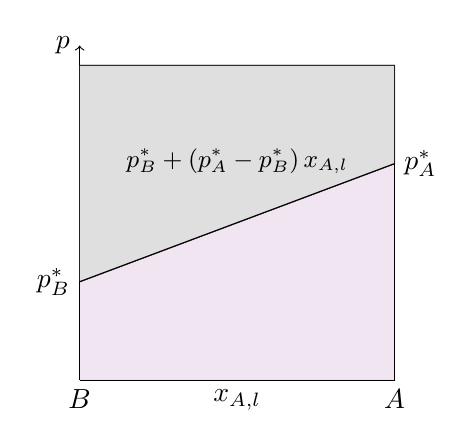
\begin{tikzpicture}
    \draw[-] (0,0) -- (4,0);
    \draw[->] (0,0) -- (0,4.25) node[left]{$p$};
    \draw[-] (4,0) -- (4,4);
    \draw[-] (0,4) -- (4,4);
    \node[below] at (0,0) {$B$};
    \node[below] at (4,0) {$A$};
    \node[below] at (2,0) {$x_{A,\l}$};
    \filldraw[fill=lightgray,opacity=0.5] (0,1.25) -- (4,2.75) -- (4,4) -- (0,4);
    \filldraw[fill=violet,opacity=0.1] (0,1.25) -- (4,2.75) -- (4,0) -- (0,0);
    \node[left] at (0,1.25) {$p_B^\ast$};
    \node[right] at (4,2.75) {$p_A^\ast$};
    \node[above] at (2,2.5) {\small{$p_B^\ast+\left(p_A^\ast-p_B^\ast\right)x_{A,\l}$}};
    \draw[-] (0,1.25) -- (4,2.75);
    
\end{tikzpicture}
\end{document}
    \end{center}
    其中上面灰色的部分为液相,下面紫色的部分为气相.可以看到,选取某组分在液相中的摩尔分数$x_\l$和压力$p$,%
    作出的理想溶液相图中两相的分界线为直线.\\
    显而易见的,两种组分在气相中的含量与它们在液相中的含量并不相同.我们有
    \[x_{A,\g}=\dfrac{p_A}{p}=\dfrac{p_A^\ast x_{A,\l}}{p_B^\ast+\left(p_A^\ast-p_B^\ast\right)x_{A,\l}}\]
    于是
    \[x_{A,\l}=\dfrac{p_B^\ast x_{A,\g}}{p_A^\ast+\left(p_B^\ast-p_A^\ast\right)x_{A,\g}}\]
    从而
    \[p=p_B^\ast+\dfrac{p_B^\ast x_{A,\g}\left(p_A^\ast-p_B^\ast\right)}{p_A^\ast+\left(p_B^\ast-p_A^\ast\right)x_{A,\g}}
    =\dfrac{p_A^\ast p_B^\ast}{p_A^\ast+\left(p_B^\ast-p_A^\ast\right)x_{A,\g}}\]
    我们以$x_{A,\g}$为横轴,$p$为纵轴,可以得到如下的相图.
    \begin{center}
        \documentclass{standalone}
\usepackage{PhysicalChemistryNote}
\begin{document}
\begin{tikzpicture}
    \draw[-] (0,0) -- (4,0);
    \draw[->] (0,0) -- (0,4.25) node[left]{$p$};
    \draw[-] (4,0) -- (4,4);
    \draw[-] (0,4) -- (4,4);
    \node[below] at (0,0) {$B$};
    \node[below] at (4,0) {$A$};
    \node[below] at (2,0) {$x_{A,\g}$};
    \draw[domain=0:4] plot[smooth](\x,{4*1.25*2.75/(11-1.5*\x)});
    \filldraw[fill=lightgray,opacity=0.5,domain=0:4] plot[smooth](\x,{4*1.25*2.75/(11-1.5*\x)}) -- (4,4) -- (0,4);
    \filldraw[fill=violet,opacity=0.1,domain=0:4] plot[smooth](\x,{4*1.25*2.75/(11-1.5*\x)}) -- (4,0) -- (0,0);
    \node[left] at (0,1.25) {$p_B^\ast$};
    \node[right] at (4,2.75) {$p_A^\ast$};
    \node[below] at (2,1.5) {\small{$\dfrac{p_A^\ast p_B^\ast}{p_A^\ast+\left(p_B^\ast-p_A^\ast\right)x_{A,\g}}$}};
    
    
\end{tikzpicture}
\end{document}
    \end{center}
    可以看到,以气相中$A$的摩尔分数作出的相图的分界线是一条下凹的曲线,总是处于液相线之下.如果我们把两条线画在同一张图中,就有
    \begin{center}
        \documentclass{standalone}
\usepackage{PhysicalChemistryNote}
\begin{document}
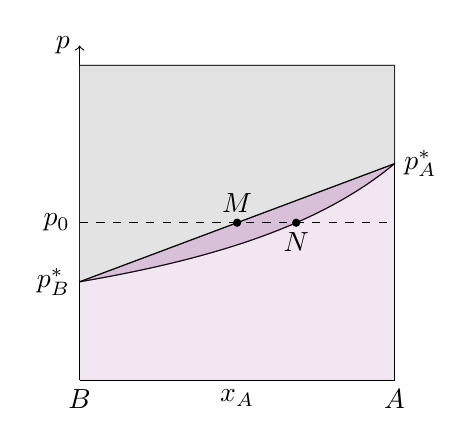
\begin{tikzpicture}
    \draw[-] (0,0) -- (4,0);
    \draw[->] (0,0) -- (0,4.25) node[left]{$p$};
    \draw[-] (4,0) -- (4,4);
    \draw[-] (0,4) -- (4,4);
    \node[below] at (0,0) {$B$};
    \node[below] at (4,0) {$A$};
    \node[below] at (2,0) {$x_{A}$};
    \draw[domain=0:4] plot[smooth](\x,{4*1.25*2.75/(11-1.5*\x)});
    \filldraw[fill=lightgray,opacity=0.25,domain=0:4] plot[smooth](\x,{4*1.25*2.75/(11-1.5*\x)}) -- (4,4) -- (0,4);
    \filldraw[fill=violet,opacity=0.05,domain=0:4] plot[smooth](\x,{4*1.25*2.75/(11-1.5*\x)}) -- (4,0) -- (0,0);
    \filldraw[fill=lightgray,opacity=0.25] (0,1.25) -- (4,2.75) -- (4,4) -- (0,4);
    \filldraw[fill=violet,opacity=0.05] (0,1.25) -- (4,2.75) -- (4,0) -- (0,0);
    \filldraw[fill=violet,opacity=0.15,domain=0:4] plot[smooth](\x,{4*1.25*2.75/(11-1.5*\x)})--(0,1.25);
    \node[left] at (0,1.25) {$p_B^\ast$};
    \node[left] at (0,2) {$p_0$};
    \node[right] at (4,2.75) {$p_A^\ast$};
    \draw[-] (0,1.25) -- (4,2.75);
    \draw[dashed] (0,2) -- (4,2);
    \fill (2,2) circle (1.5pt) node[above]{$M$};
    \fill (2.75,2) circle (1.5pt) node[below]{$N$};
    
\end{tikzpicture}
\end{document}
    \end{center}
    根据相律,在两相平衡时系统的自由度为$f=C+n-\varPhi=2+2-0$,只要给定压强$p_0$和温度$T$就可以确定其组成和状态.因此,%
    我们作一条直线$p=p_0$分别交两条分界线于$M,N$两点,就可以知道此时两相平衡时液相和气相的组成.\\
    容易看出在平衡时,蒸气压大的组分在气相中的摩尔分数总是比在液相中的摩尔分数高.
\end{derivation}
通常来说,我们更常在恒定压力下对系统进行改变,例如蒸馏和精馏等操作.%
因此,$T-x$图更为常用.
\begin{derivation}\setcounter{equation}{0}
    我们仍然讨论由组分$A$和组分$B$组成的理想溶液,并保持总压力为$p$不变.\\
    根据Clausius-Clapeyron方程有
    \begin{equation}
        \dfrac{\di\ln p_{i}^\ast}{\di T}=\dfrac{\Delta_\vap H_{\m,i}}{RT^2}
    \end{equation}
    其中$i=A,B$.我们再假定摩尔蒸发焓随温度变化很小,设纯的$i$在$p$下的沸点为$T_i^\ast$,对(1)定积分有
    \begin{equation}
        \ln\dfrac{p_i^\ast}{p}=\dfrac{\Delta_\vap H_{\m,i}}{R}\left(\dfrac{1}{T_i^\ast}-\dfrac1T\right)
    \end{equation}
    移项并取指数就有
    \begin{equation}
        p_i^\ast=p\exp{\left[\dfrac{\Delta_\vap H_{\m,i}}{R}\left(\dfrac{1}{T_i^\ast}-\dfrac1T\right)\right]}
    \end{equation}
    根据Raoult定律有
    \begin{equation}
        p=p_{A}^\ast x_{A,\l}+p_B^\ast\left(1-x_{A,\l}\right)
    \end{equation}
    将(3)代入其中就有
    \begin{equation}
        x_{A,\l}\exp{\left[\dfrac{\Delta_\vap H_{\m,A}}{R}\left(\dfrac{1}{T_A^\ast}-\dfrac1T\right)\right]}
        +\left(1-x_{A,\l}\right)\exp{\left[\dfrac{\Delta_\vap H_{\m,B}}{R}\left(\dfrac{1}{T_B^\ast}-\dfrac1T\right)\right]}=1
    \end{equation}
    这就给出了$T$与$x_{A,\l}$的函数关系,绘制出的相图如下所示.
    \begin{center}
        \documentclass{standalone}
\usepackage{PhysicalChemistryNote}
\begin{document}
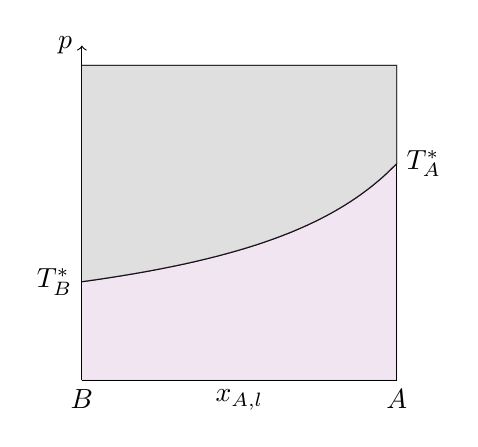
\begin{tikzpicture}
    \draw[-] (0,0) -- (4,0);
    \draw[->] (0,0) -- (0,4.25) node[left]{$p$};
    \draw[-] (4,0) -- (4,4);
    \draw[-] (0,4) -- (4,4);
    \node[below] at (0,0) {$B$};
    \node[below] at (4,0) {$A$};
    \node[below] at (2,0) {$x_{A,\l}$};
    \draw[domain=0:4] plot[smooth](\x,{1/ln(0.1967*(11.3117-\x))});
    \filldraw[fill=lightgray,opacity=0.5,domain=0:4] plot[smooth](\x,{1/ln(0.1967*(11.3117-\x))}) -- (4,4) -- (0,4);
    \filldraw[fill=violet,opacity=0.1,domain=0:4] plot[smooth](\x,{1/ln(0.1967*(11.3117-\x))}) -- (4,0) -- (0,0);
    \node[left] at (0,1.25) {$T_B^\ast$};
    \node[right] at (4,2.75) {$T_A^\ast$}; 
    
\end{tikzpicture}
\end{document}
    \end{center}
    如果将$p_A+p_B=p$和$x_{A,\g}$代入(3)可得
    \begin{equation}
        x_{A,\g}\exp{\left[\dfrac{\Delta_\vap H_{\m,A}}{R}\left(\dfrac{1}{T_A^\ast}-\dfrac1T\right)\right]}
        =\left(1-x_{A.,\g}\right)\exp{\left[\dfrac{\Delta_\vap H_{\m,B}}{R}\left(\dfrac{1}{T_B^\ast}-\dfrac1T\right)\right]}
    \end{equation}
\end{derivation}

\end{document}
\end{document}